\documentclass[french]{layout/Report}
\usepackage{layout/Report}
\usepackage{layout/ReportFrontPage}

\usepackage{pgf,tikz,textcomp}
\usepackage[section]{placeins}
\usepackage{romannum}
\usetikzlibrary{arrows}
\usepackage{mathtools}
\usepackage{array}
\usepackage{color}
\usepackage{graphicx}
\usepackage{todonotes}
\usepackage{enumitem}
\usepackage{MnSymbol} % rectangle symbol
\usepackage{pdfpages} % for appendix

\DeclarePairedDelimiter\abs{\lvert}{\rvert}%

\begin{document}

\pagenumbering{arabic}


\frontpage{Télécommande à 1 canal par infrarouge}
%-------------------------------------------------------------------------------
\section{Introduction}
Le but est de concevoir un système d'émission - réception infrarouge avec adressage
permettant d'enclencher et déclencher un relais optique.

%-------------------------------------------------------------------------------
\section{Structure générale et principe}

Le système est divisé en 5 étages pour faciliter le développement et la testabilité:

\begin{description}[leftmargin=!,labelwidth=4cm, labelindent=\parindent]
	\item[Générateur de signal] Générateur de salves espacées de $\tau = \SI{100}{\milli\second}$ formée par $n_{pulse}$ impulsions de durée $t_0 =  \SI{100}{\micro\second}$ avec une période $T_0 = \SI{1}{\milli\second}$. 
\item[LED driver] Sortie de puissance qui contrôle la LED IR.
\item[Récepteur] Récepteur IR avec amplification et filtrage. La sortie est le signal digital des impulsions.
\item[Décodeur] Circuit logique de décodage du nombre d'impulsions. La sortie est une impulsion de $t_{true} = \SI{5}{\milli\second}$ pour chaque salve correcte reçue.
\item[Sortie] Circuit de détection d'interruption du signal avec commutation et du relais optique.
\end{description}

\begin{figure}[H]
\centering
\vspace{5mm}
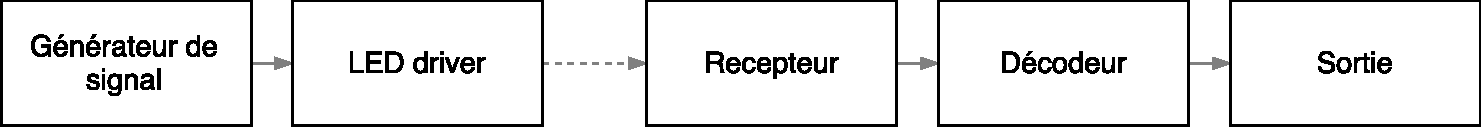
\includegraphics[width=\textwidth]{fig/IRemote_schema_structure}
\caption{Schéma bloc du système avec signaux}
\label{fig:schema_bloc}
\vspace{5mm}
\end{figure}

%-------------------------------------------------------------------------------
\section{Notation et nomenclature}

\begin{center}
	\begin{tabular}{| c | l | l |}
		\hline
		$n_{pulse}$	& Nombre d'impulsion dans une salve (addressage) & $13$ \\ \hline
		$t_0$				& Durée high d'une impulsion & $\SI{0.1}{\milli\second}$	\\ \hline
		$T_0$				& Période des impulsions& $\SI{1.0}{\milli\second}$	\\ \hline
		$D_0$				& Duty cycle dans une salve & $10\%$	\\ \hline
		$\tau$			& Période des slaves	& $\SI{0.1}{\second}$\\ \hline
		$t_{miss}$  & Durée pour la détection d'une impulsion manquante & $\SI{1.8}{\milli\second}$ \\ \hline
		$t_{true}$  & Durée signal une salve correcte & \SI{5}{\milli\second}\\ \hline
	\end{tabular}
\end{center}

\section{Dimensionnements}
\subsection{Signal}
Le nombre d'impulsions $n_{pulse}$ a été fixé arbitrairement à 13. La période et le duty-cycle des impulsions sont dictés par ce que la LED infrarouge peut supporter (c.f. \ref{subsec:LED_driver}).

\subsection{Générateur de signal}
Le générateur de signal génère dans OUTPUT des salves de $n_{pulses} = 13$ à une période $\tau = \SI{0.1}{\second}$ en active high tant que celui-ci est alimenté à 3V. Les impulsions dans les salves ont une durée high $t_0 = \SI{0.1}{\milli\second}$ et une période $T_0 = \SI{1.0}{\milli\second}$. Le nombre d'impulsions et les durées ne sont pas garanties lorsque l'alimentation est retirée.

\begin{description}[leftmargin=!,labelwidth=3cm, labelindent=\parindent]
	\item[Pulse timer] Génère des impulsions à hautes fréquences tant qu'il n'est pas RESET. Il est formé d'un timer TLC555 en configuration bascule astable. Les dimensionnements sont fait selon le datasheet \cite{TLC555} avec une capacité $\mathit{C16} = \SI{100}{\nano F}$ choisie petite pour la simplicité et la limitation de la consommation.
		\begin{equation*}
			\begin{cases}
				t_0 = 0.693(\mathit{R20}+\mathit{R23})\mathit{C16} \\
				T_0 = 0.693(\mathit{R20}+2\mathit{R23})\mathit{C16} \\
			\end{cases}
			\quad\Rightarrow\quad
			\begin{cases}
				\mathit{R20} = \SI{12}{\kilo\ohm} \\
				\mathit{R23} = \SI{1.5}{\kilo\ohm}
			\end{cases}
		\end{equation*}

        \begin{figure}[H]
        \centering
        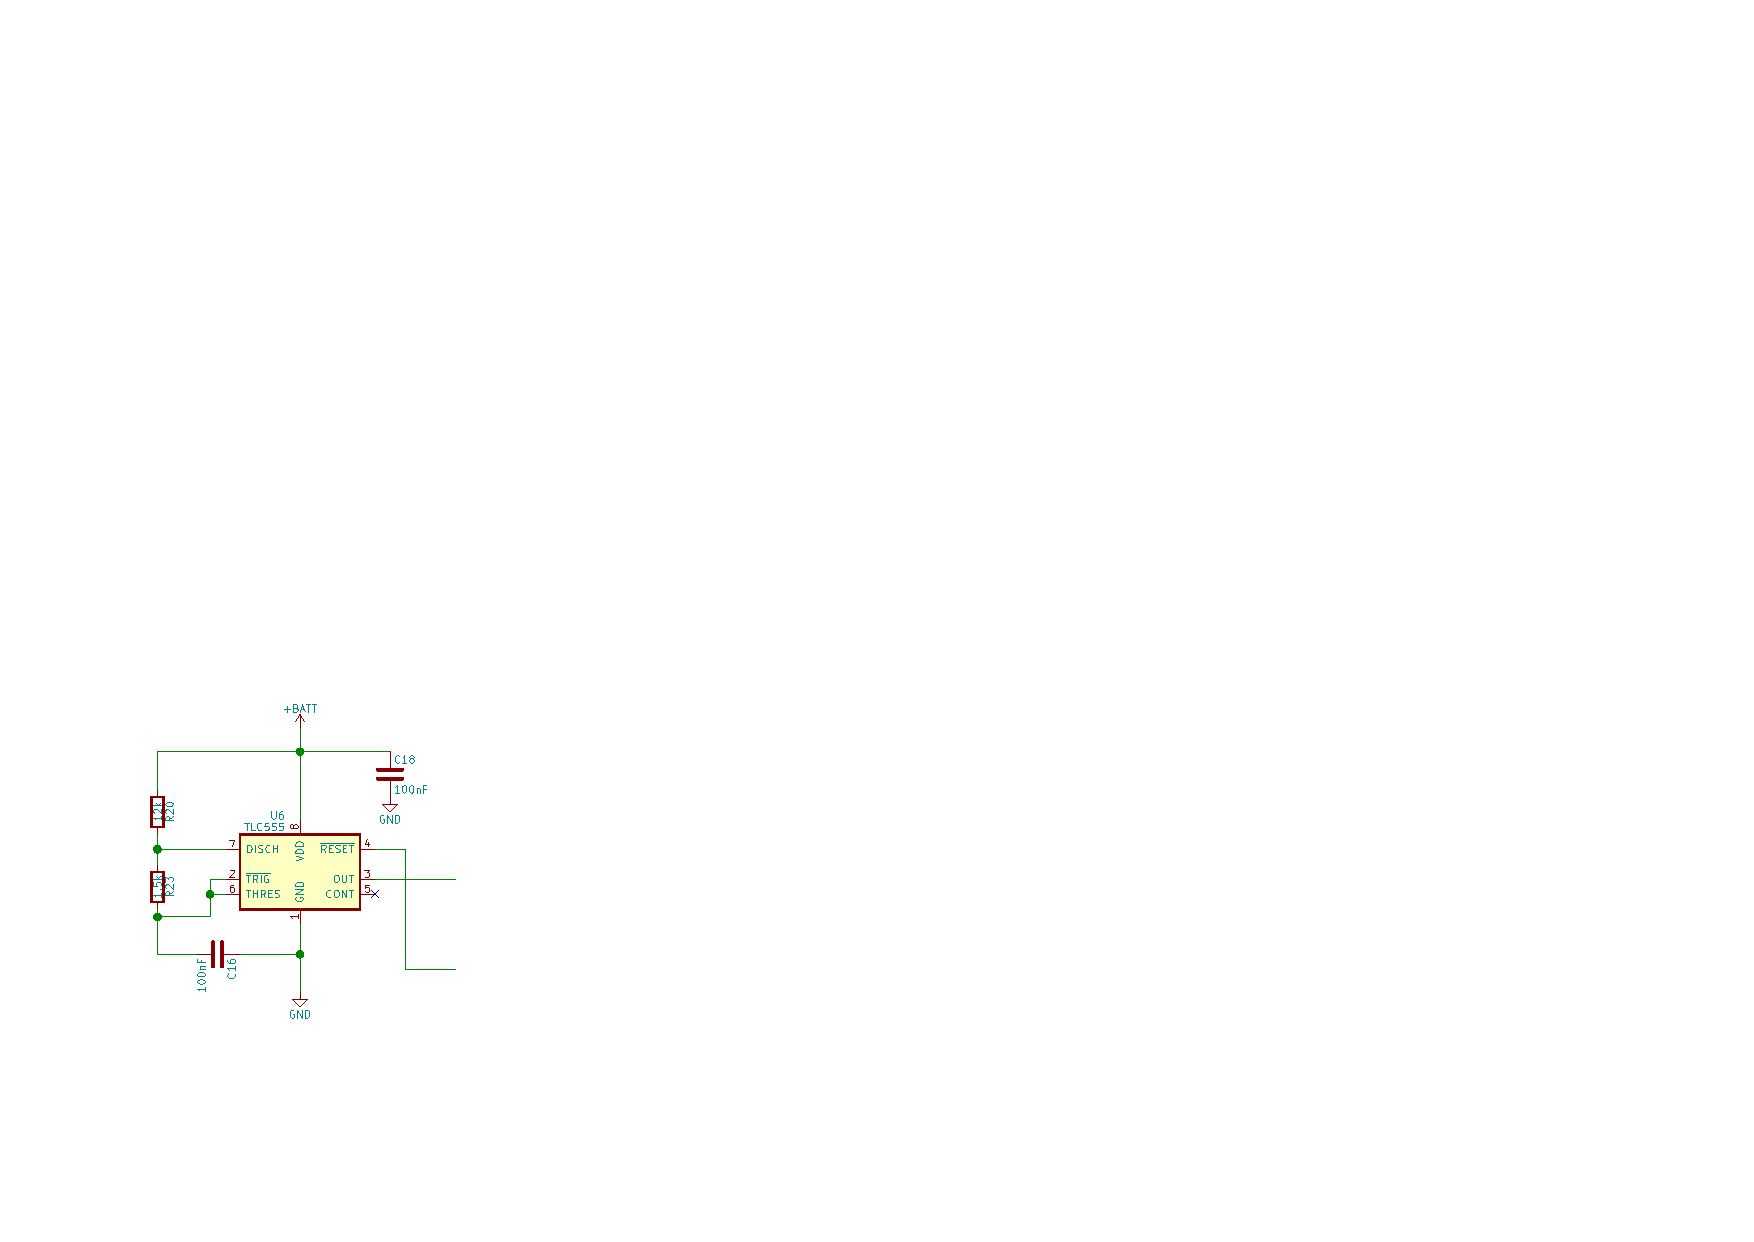
\includegraphics[width=0.3\textwidth]{fig/pulse_timer.pdf}
        \end{figure}

	\item[Down counter] Compte le nombre d'impulsions reçues depuis son dernier RESET et maintient le RESET du pulse timer le bloquant ainsi lorsque $n_{pulse}$ impulsions ont été reçues. Il est formé d'un compteur HEF4526B \cite{HEF4526B}.

	\item[Burst timer] Réinitialise le down counter à une période $\tau = \SI{0.1}{\second}$ pour recommencer une salve. Il est formé d'un timer TLC555 en configuration bascule astable. Les dimensionnements sont fait selon le datasheet \cite{TLC555} avec une capacité $\mathit{C10} = \SI{100}{\nano F}$ choisie petite pour la simplicité et la diminution de la consommation. La durée high doit être plus grand que la durée durée d'une salve.
		\begin{equation*}
			\begin{cases}
				\tau = 0.693(\mathit{R13}+2\mathit{R19})\mathit{C10} \\
				n_{pulse}*\frac{T_0}{\tau} < \frac{\mathit{R13}+\mathit{R19}}{\mathit{R13}+2\mathit{19}} \\
			\end{cases}
		\quad\Rightarrow\quad
			\begin{cases}
				\mathit{R13} = \SI{556}{\kilo\ohm} \\
				\mathit{R19} = \SI{467}{\kilo\ohm} \\
			\end{cases}
		\end{equation*}

        \begin{figure}[H]
        \centering
        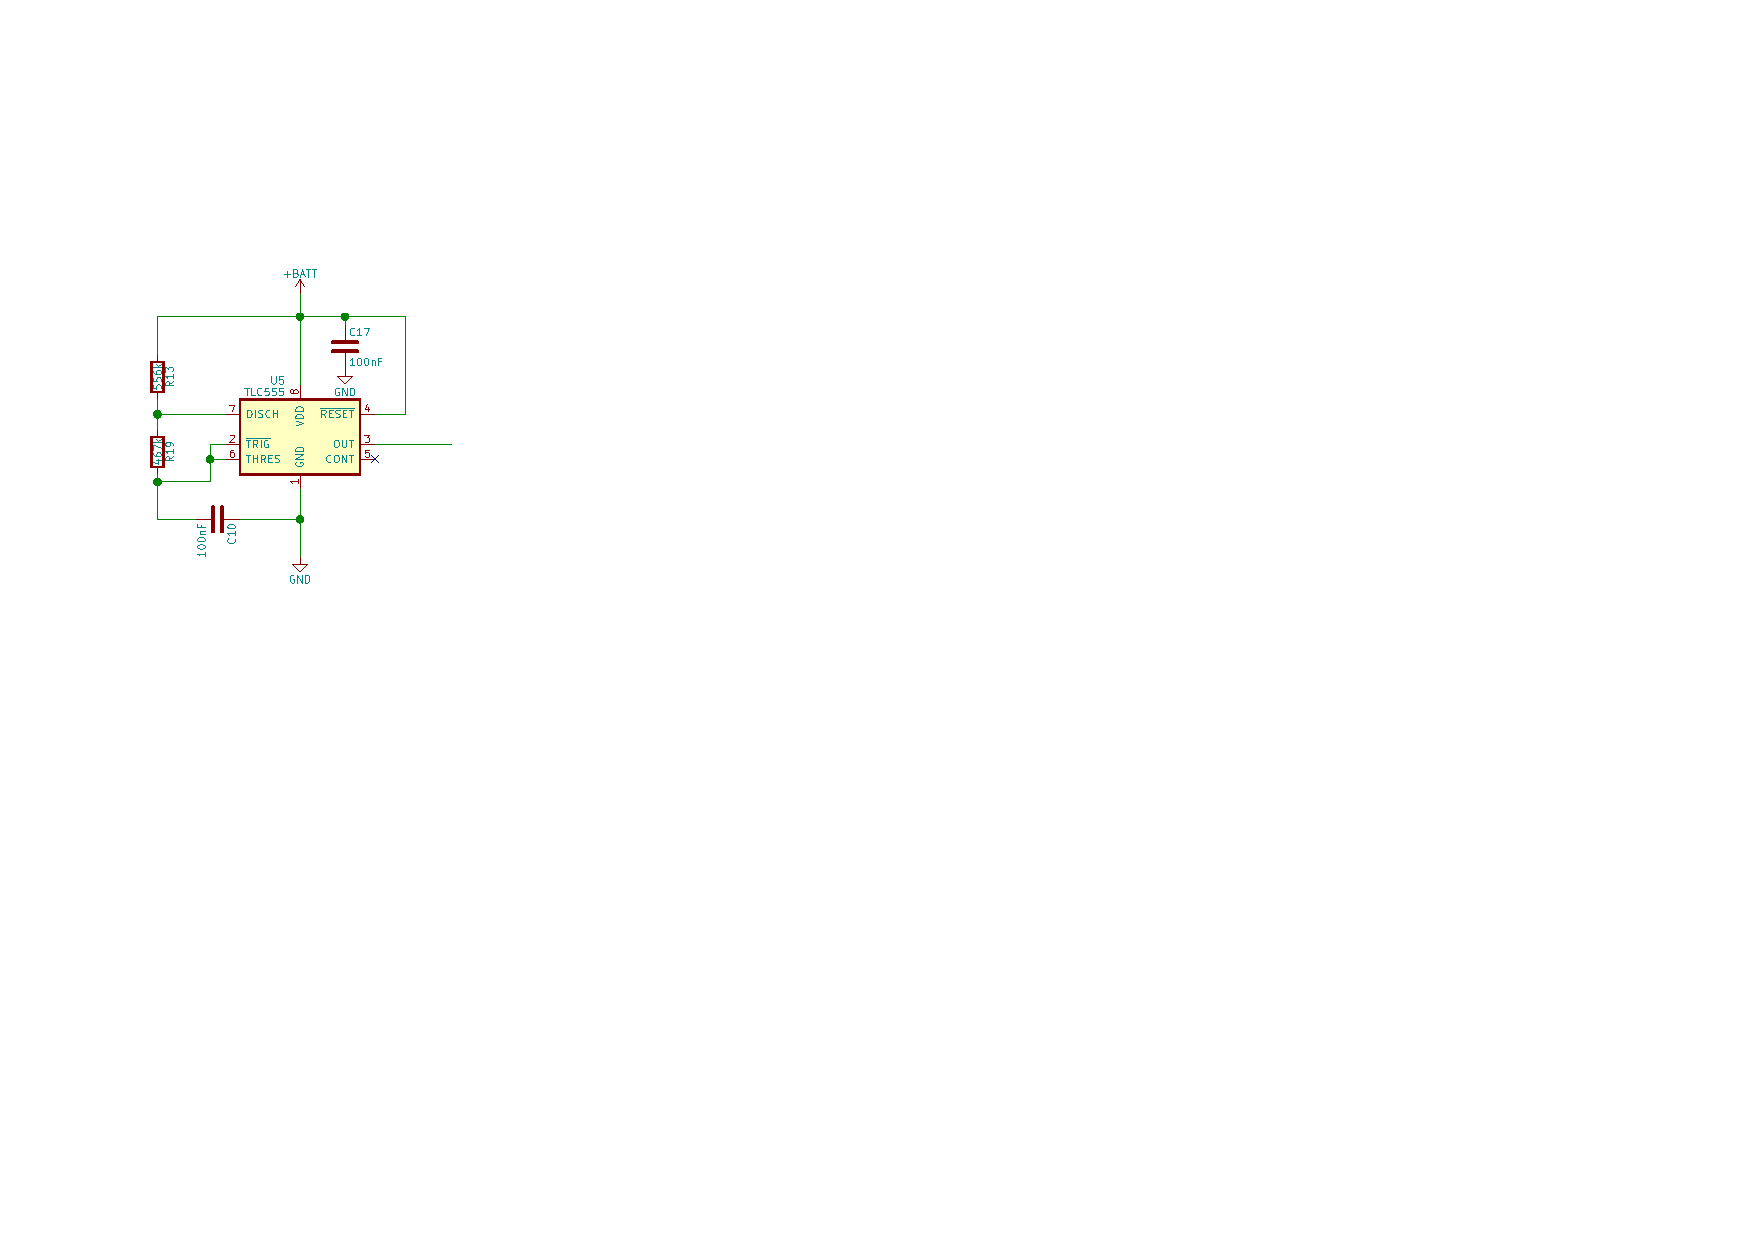
\includegraphics[width=0.3\textwidth]{fig/burst_timer.pdf}
        \end{figure}

	\item[Logic] Assure les conditions logiques sur les signaux. Il est formée d'un quadruple 2-input NOR HEF4001 \cite{HEF4001B}.
\end{description}

\subsection{LED driver}
\label{subsec:LED_driver}
Le LED driver allume la LED infrarouge lorsque LED\_SIGNAL est high. Il assure une bonne émission de la LED sans l'endommager si le signal de 3V a une période $T_0 = \SI{1}{\milli\second}$ avec un duty-cycle $D_0 = 10\%$.

La LED est une LD271(H). Selon son datasheet \cite{LD271(H)}, celle-ci accepte $\SI{1}{\ampere}$ durant $\SI{0.1}{\milli\second}$ toutes les $\SI{1.0}{\milli\second}$. Ce sont ses valeurs qui ont dicté le choix du signal. Le courant est limité par la résistance $\mathit{R14} = \SI{1}{\ohm}$. 
La tension au borne de la résistance $\mathit{R14}$ a été mesurée pour vérifier que le courant dans la LED ne dépasse pas $\SI{1}{\ampere}$.
L'alimentation se fait par le transistor NMOS IRLU8259\cite{IRLU8259} avec une faible tension Drain-Source.

La capacité de découplage est dimensionnée pour limiter la baisse de tension à 0.3V pendant une impulsion de durée $t_0 = \SI{0.1}{\milli\second}$ pour assurer la puissance de l'émission.
\begin{equation*}
	\mathit{C7} \ge \frac{I_{max}*t_0}{\Delta V_{max}} = \frac{\SI{1}{\ampere}*\SI{100}{\micro\second}}{\SI{0.3}{\volt}} = \SI{333}{\micro\farad} \Rightarrow \SI{470}{\micro\farad}
\end{equation*}

% \begin{figure}[H]
% \centering
% 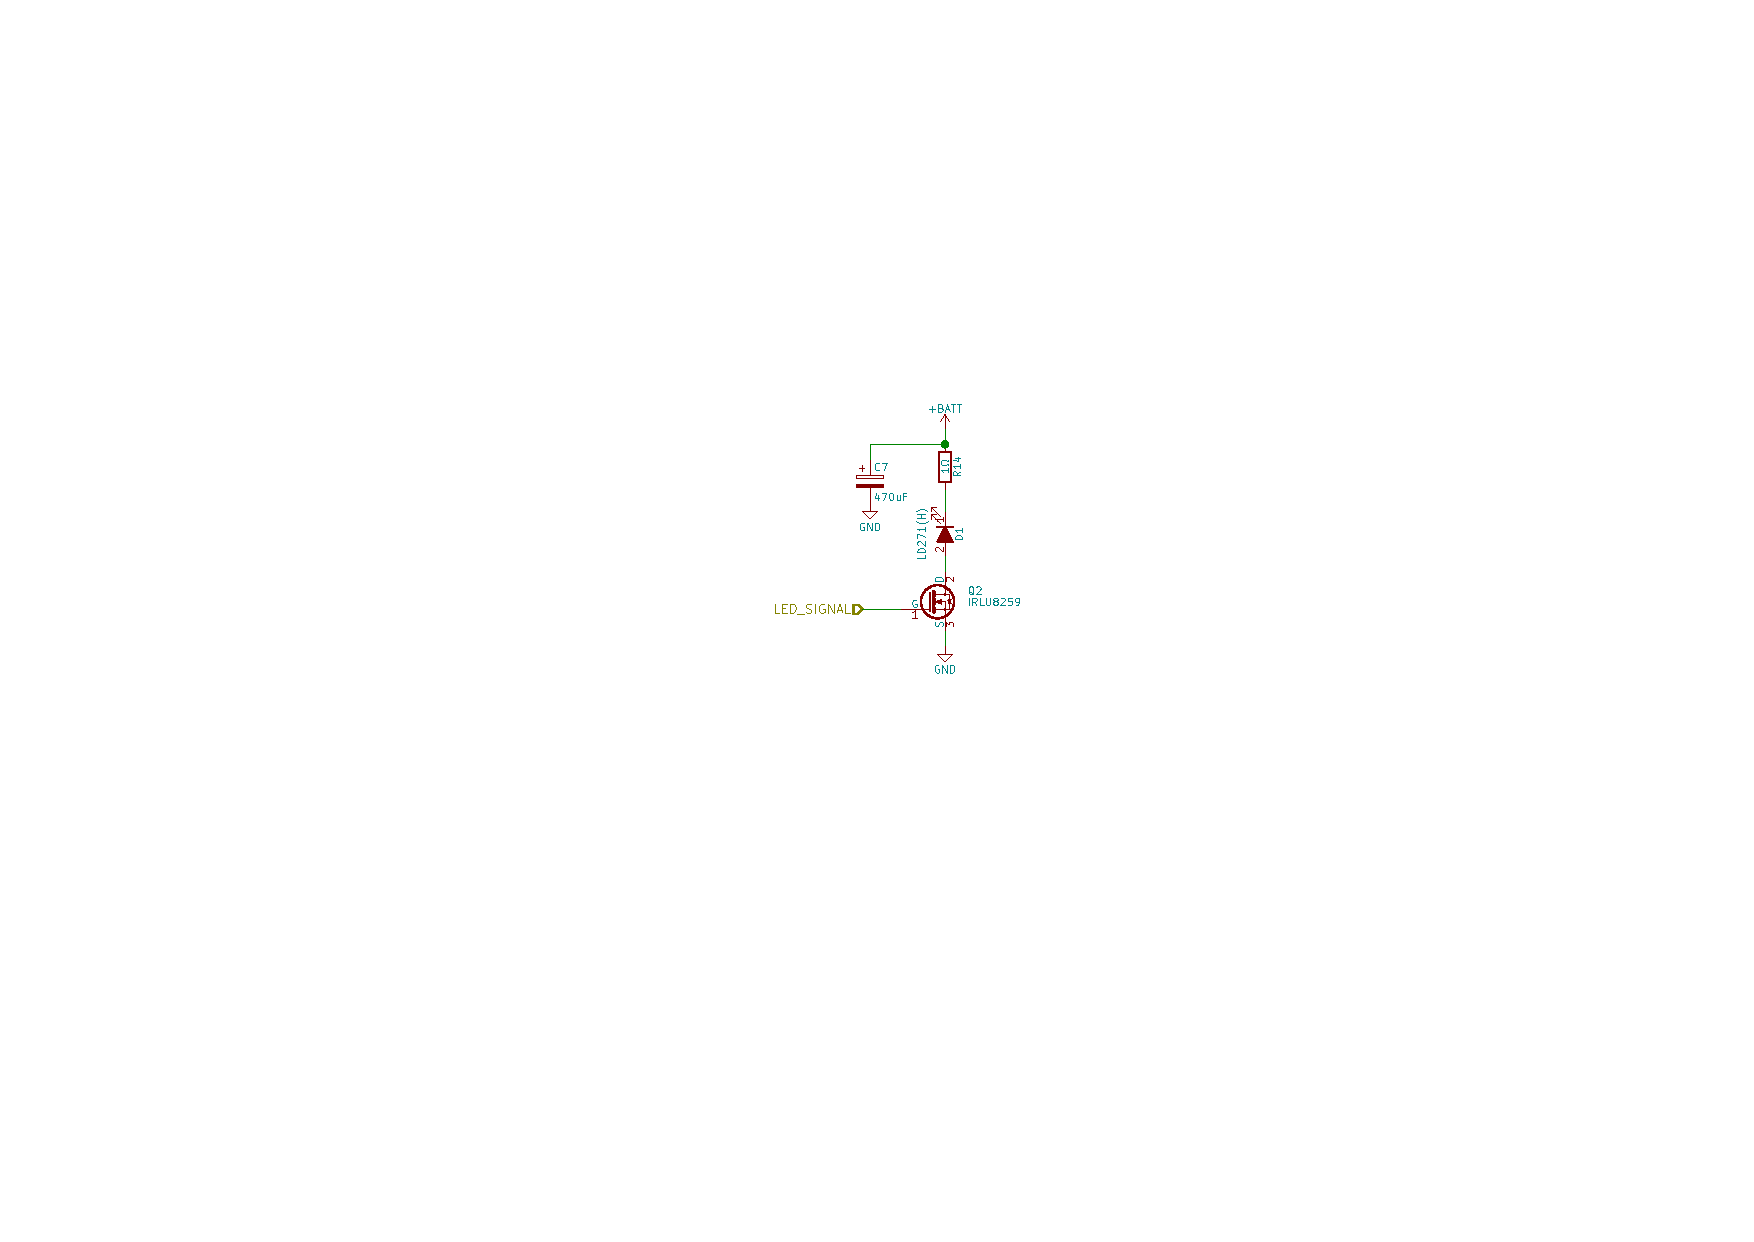
\includegraphics[width=0.3\textwidth]{fig/ir_led.pdf}
% \end{figure}

\subsection{Récepteur et filtrage}
Cet étage est composé de 3 sous-étages en série.

\begin{description}[leftmargin=!,labelwidth=3cm, labelindent=\parindent]
	\item[Convertisseur]
		La photodiode génère un petit courant qui est converti en une tension par l'amplificateur opérationnel LMC6482\cite{LMC6482}.
		La résistance $\mathit{R15}$ définit le gain et est assez élevée car le courant est relativement faible.
		Dans le conditions de test, une valeur de $\SI{1}{\mega\ohm}$ donnait les meilleures résultâts.
		En outre, la capacité $\mathit{C8} = \SI{10}{\pico\farad}$ filtre le bruit de haute fréquences d'ordre de $\SI{100}{\kilo Hz}$.

		\begin{figure}[H]
			\centering
			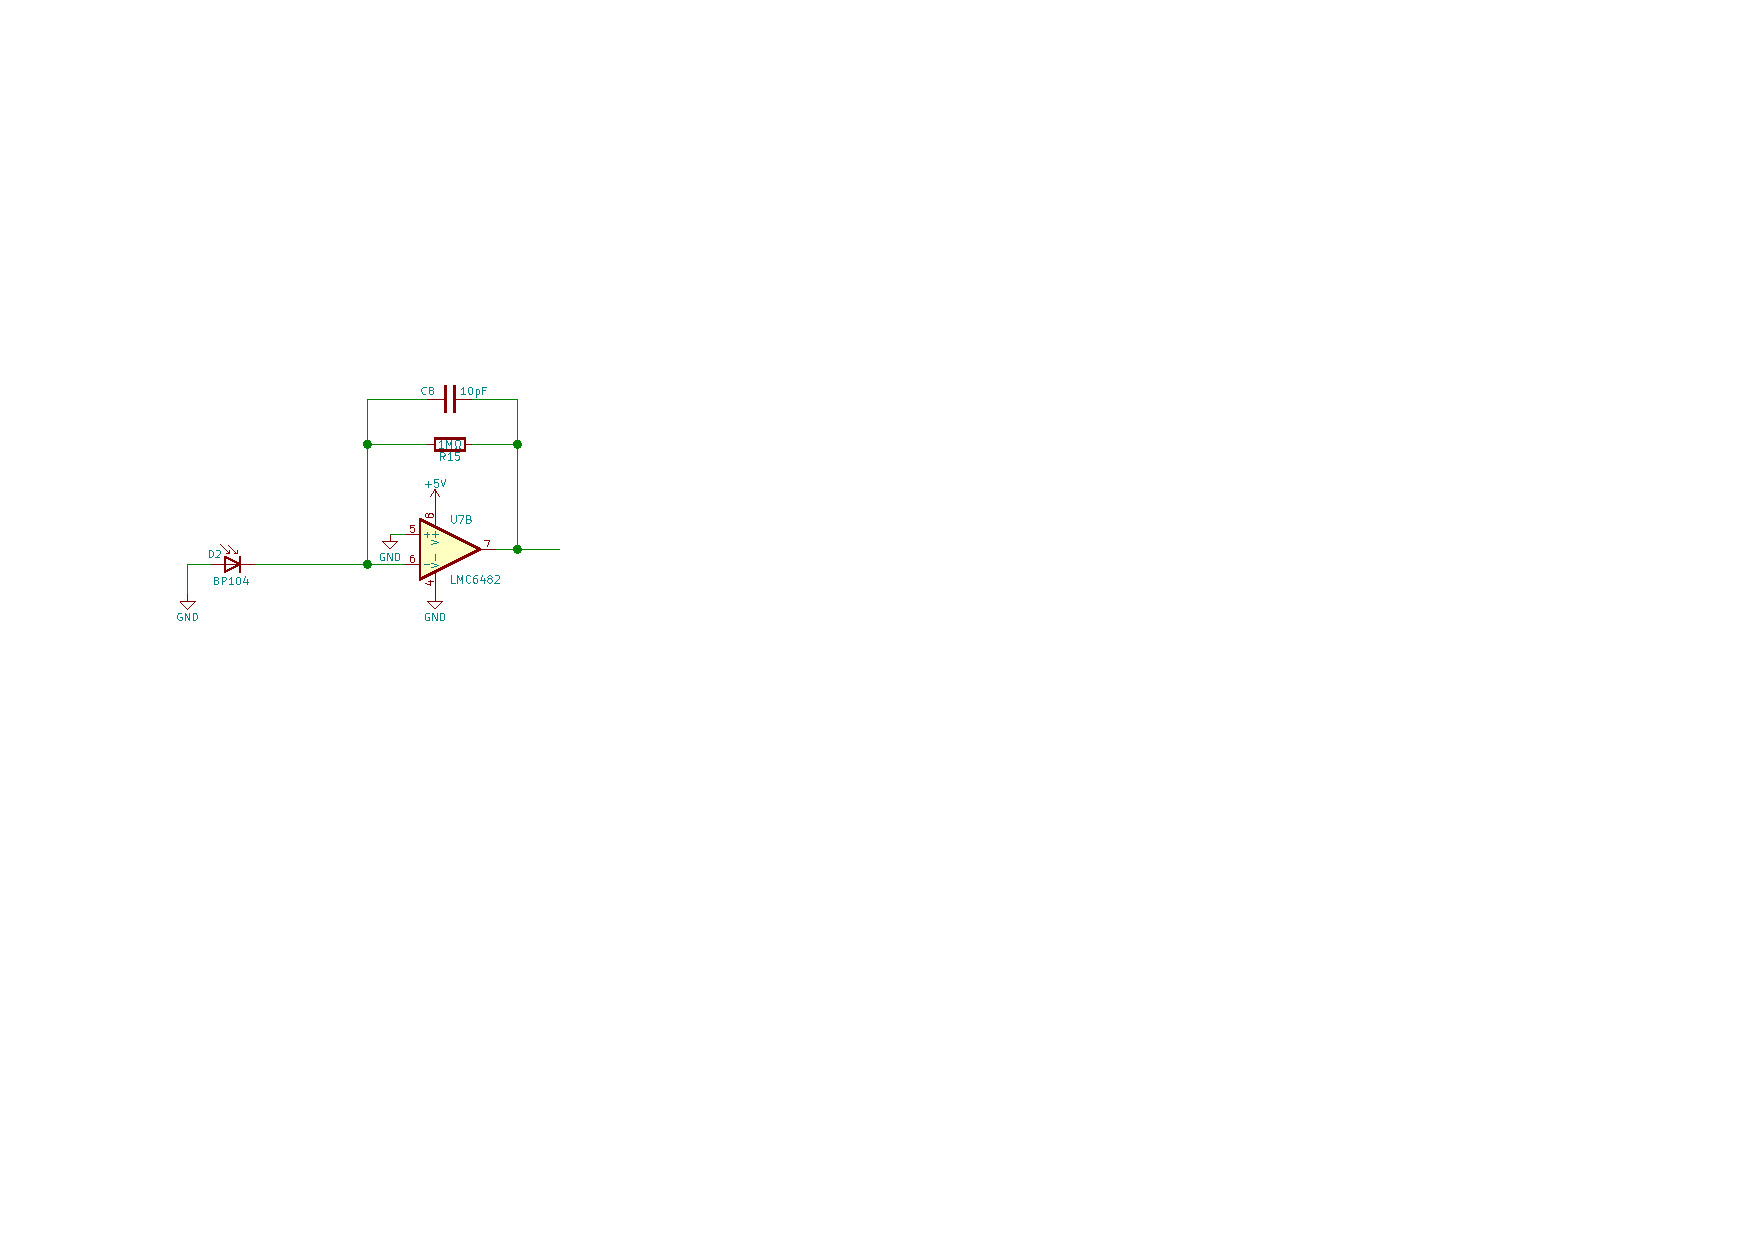
\includegraphics[width=0.4\textwidth]{fig/current_to_voltage_converter.pdf}
		\end{figure}

	\item[Amplificateur] Convertit le petit courant de la diode en tension tout en appliquant un filtre passe-bas.
		\todo[inline]{wrong text at "Amplificateur"}

		\begin{figure}[H]
			\centering
			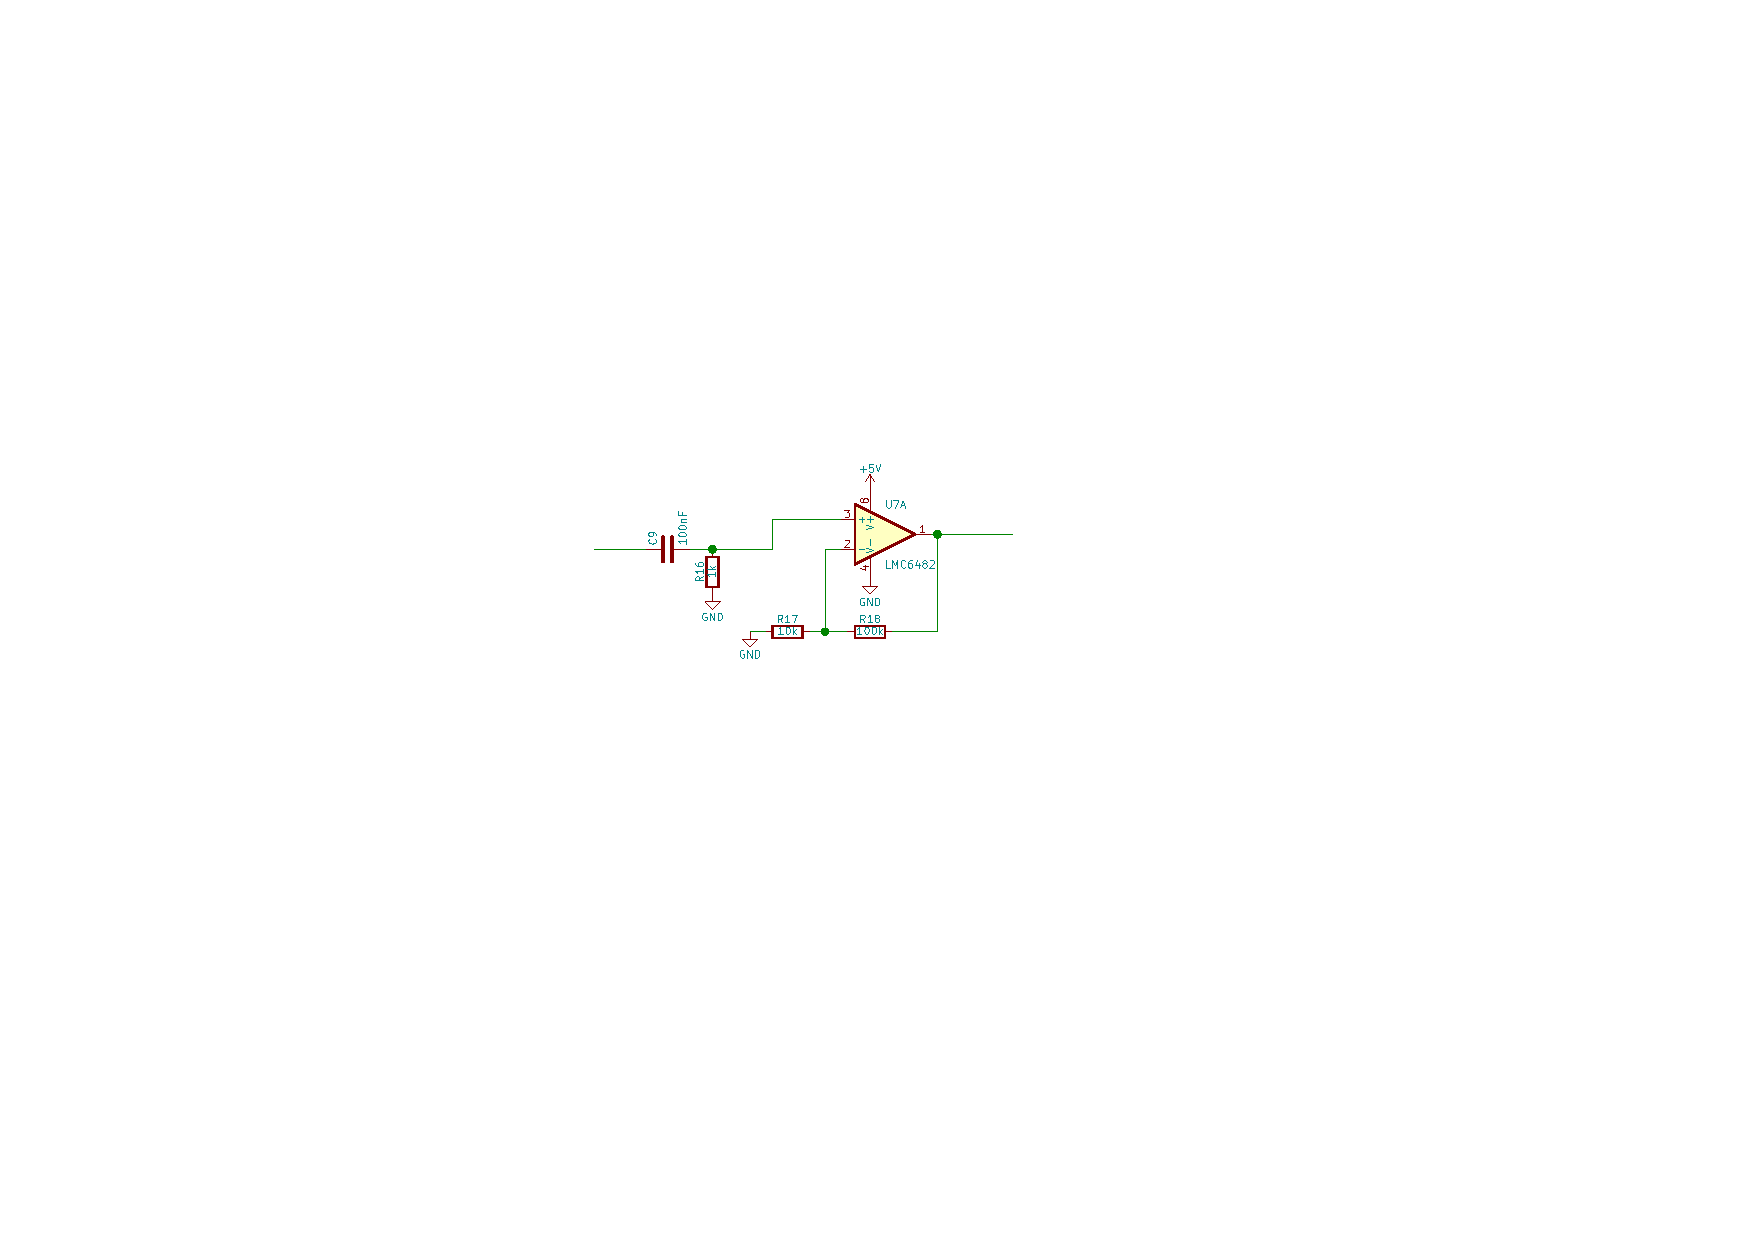
\includegraphics[width=0.4\textwidth]{fig/amplifier.pdf}
		\end{figure}

	\item[Schmitt trigger] Génère un signal carré avec 2 seuils: $V_+ = \SI{4.05}{\volt}$ et $V_- = \SI{2.02}{\volt}$. Les valeurs de ces seuils ont été choisis arbitrairement pour être comprises entre $\SI{0}{\volt}$ et $\SI{5}{\volt}$ et supérieures au bruit. Le choix des résistances ayant un degrés de liberté, celles-ci ont été choisies relativement grandes pour diminuer la consommation. La résistance $\mathit{R21}$ n'est qu'une résistance de pull-up choisie à $\SI{10}{\kilo\ohm}$.
	\todo[inline]{R21 vraiment utiles?}	
	\begin{equation*}
		\begin{cases}
			V_+ = \frac{1}{1+\frac{\mathit{R9}*\mathit{R11}}{\mathit{R10}*(\mathit{R9+\mathit{R11})}}} \\
			V_- = \frac{1}{1+\frac{\mathit{R9}*(\mathit{R10}+\mathit{R11})}{\mathit{R10}*\mathit{R11}}} \\
		\end{cases}
		\Rightarrow\quad
		\begin{cases}
			\mathit{R9}  = \SI{4.7}{\kilo\ohm} \\
			\mathit{R10} = \SI{10.0}{\kilo\ohm} \\
			\mathit{R11} = \SI{4.7}{\kilo\ohm} \\
		\end{cases}
		\end{equation*}

        \begin{figure}[H]
        \centering
        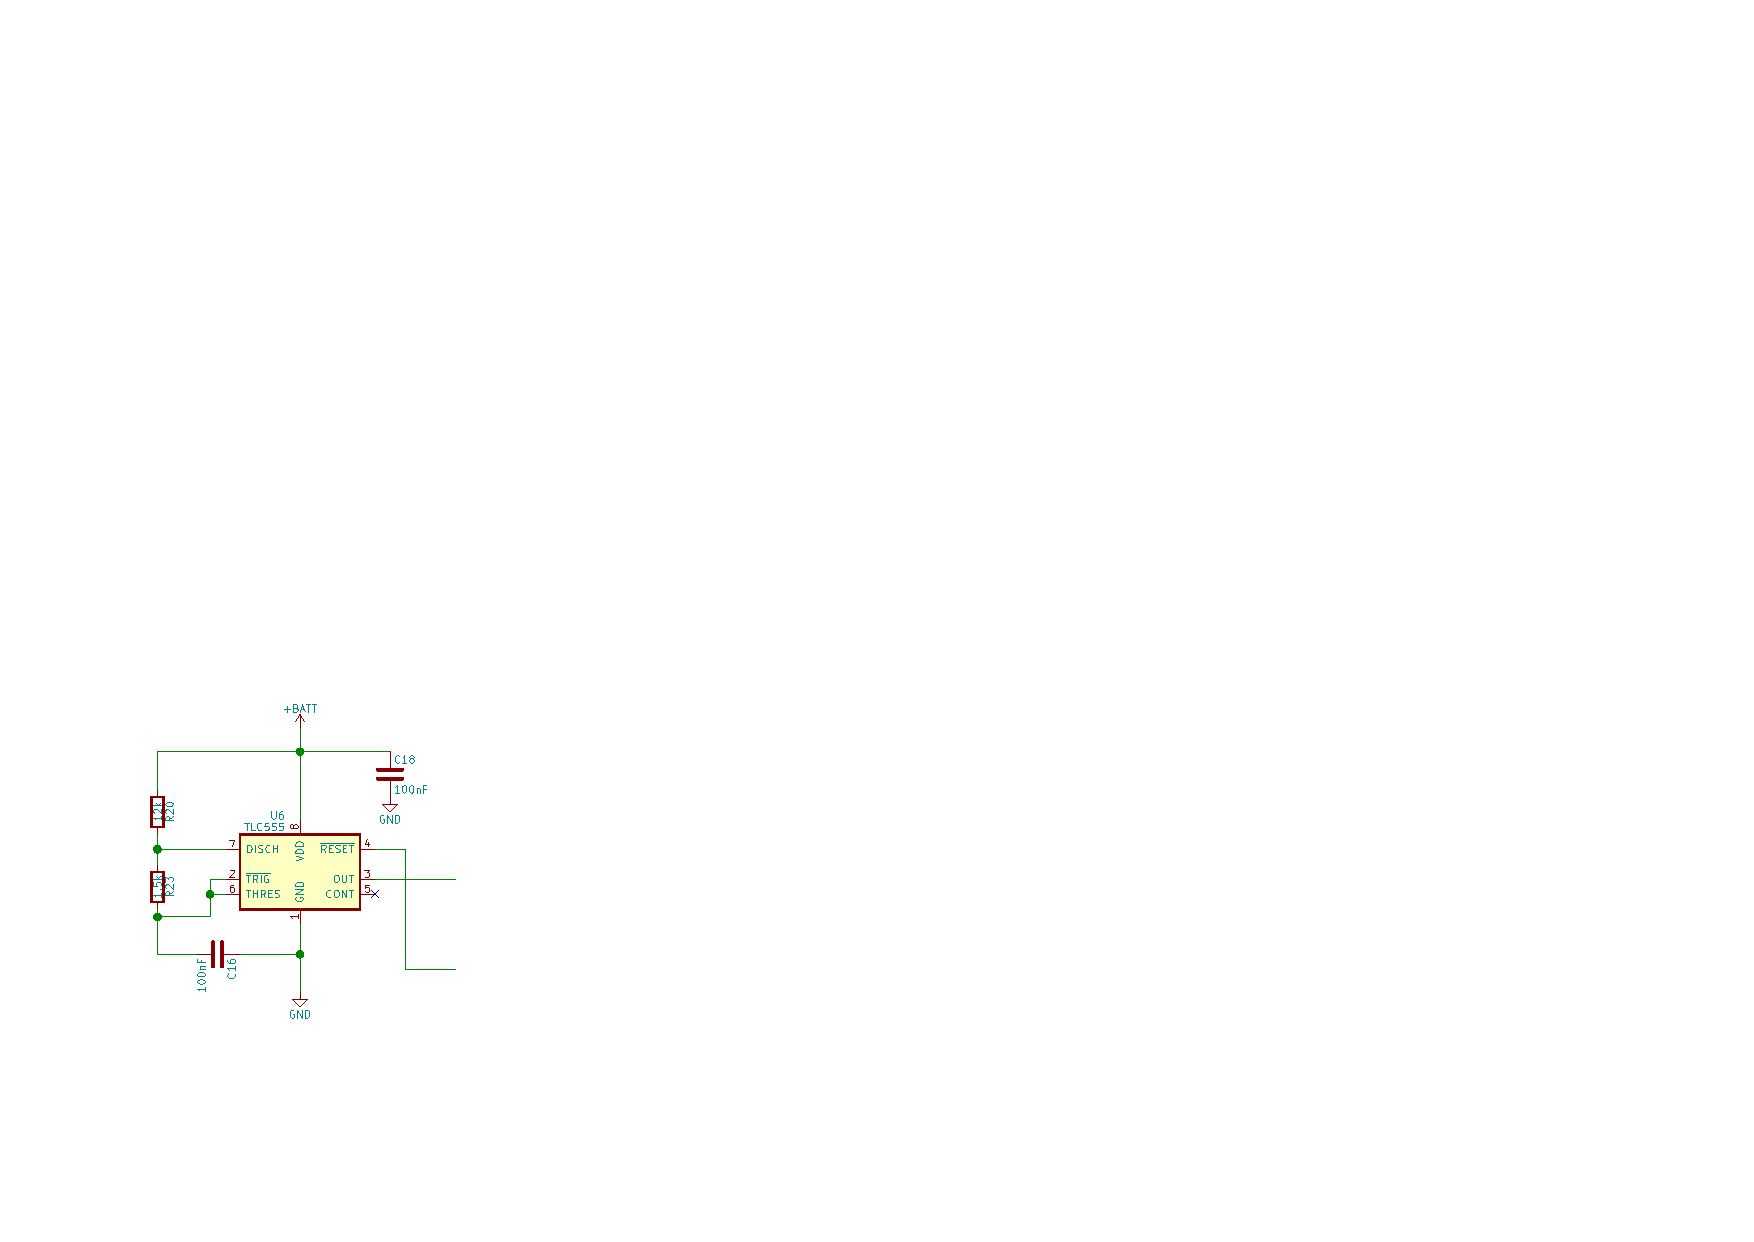
\includegraphics[width=0.3\textwidth]{fig/pulse_timer.pdf}
        \end{figure}

	\item[Down counter] Compte le nombre d'impulsions reçues depuis son dernier RESET et maintient le RESET du pulse timer le bloquant ainsi lorsque $n_{pulse}$ impulsions ont été reçues. Il est formé d'un compteur HEF4526B \cite{HEF4526B}.

	\item[Burst timer] Réinitialise le down counter à une période $\tau = \SI{0.1}{\second}$ pour recommencer une salve. Il est formé d'un timer TLC555 en configuration bascule astable. Les dimensionnements sont fait selon le datasheet \cite{TLC555} avec une capacité $\mathit{C10} = \SI{100}{\nano F}$ choisie petite pour la simplicité et la limitation de la consommation. La durée high doit être plus grand que la durée durée d'une salve.
		\begin{equation*}
			\begin{cases}
				\tau = 0.693(\mathit{R13}+2\mathit{R19})\mathit{C10} \\
				n_{pulse}*\frac{T_0}{\tau} < \frac{\mathit{R13}+\mathit{R19}}{\mathit{R13}+2\mathit{19}} \\
			\end{cases}
		\quad\
		\
	\end{equation*}

		\begin{figure}[H]
			\centering
			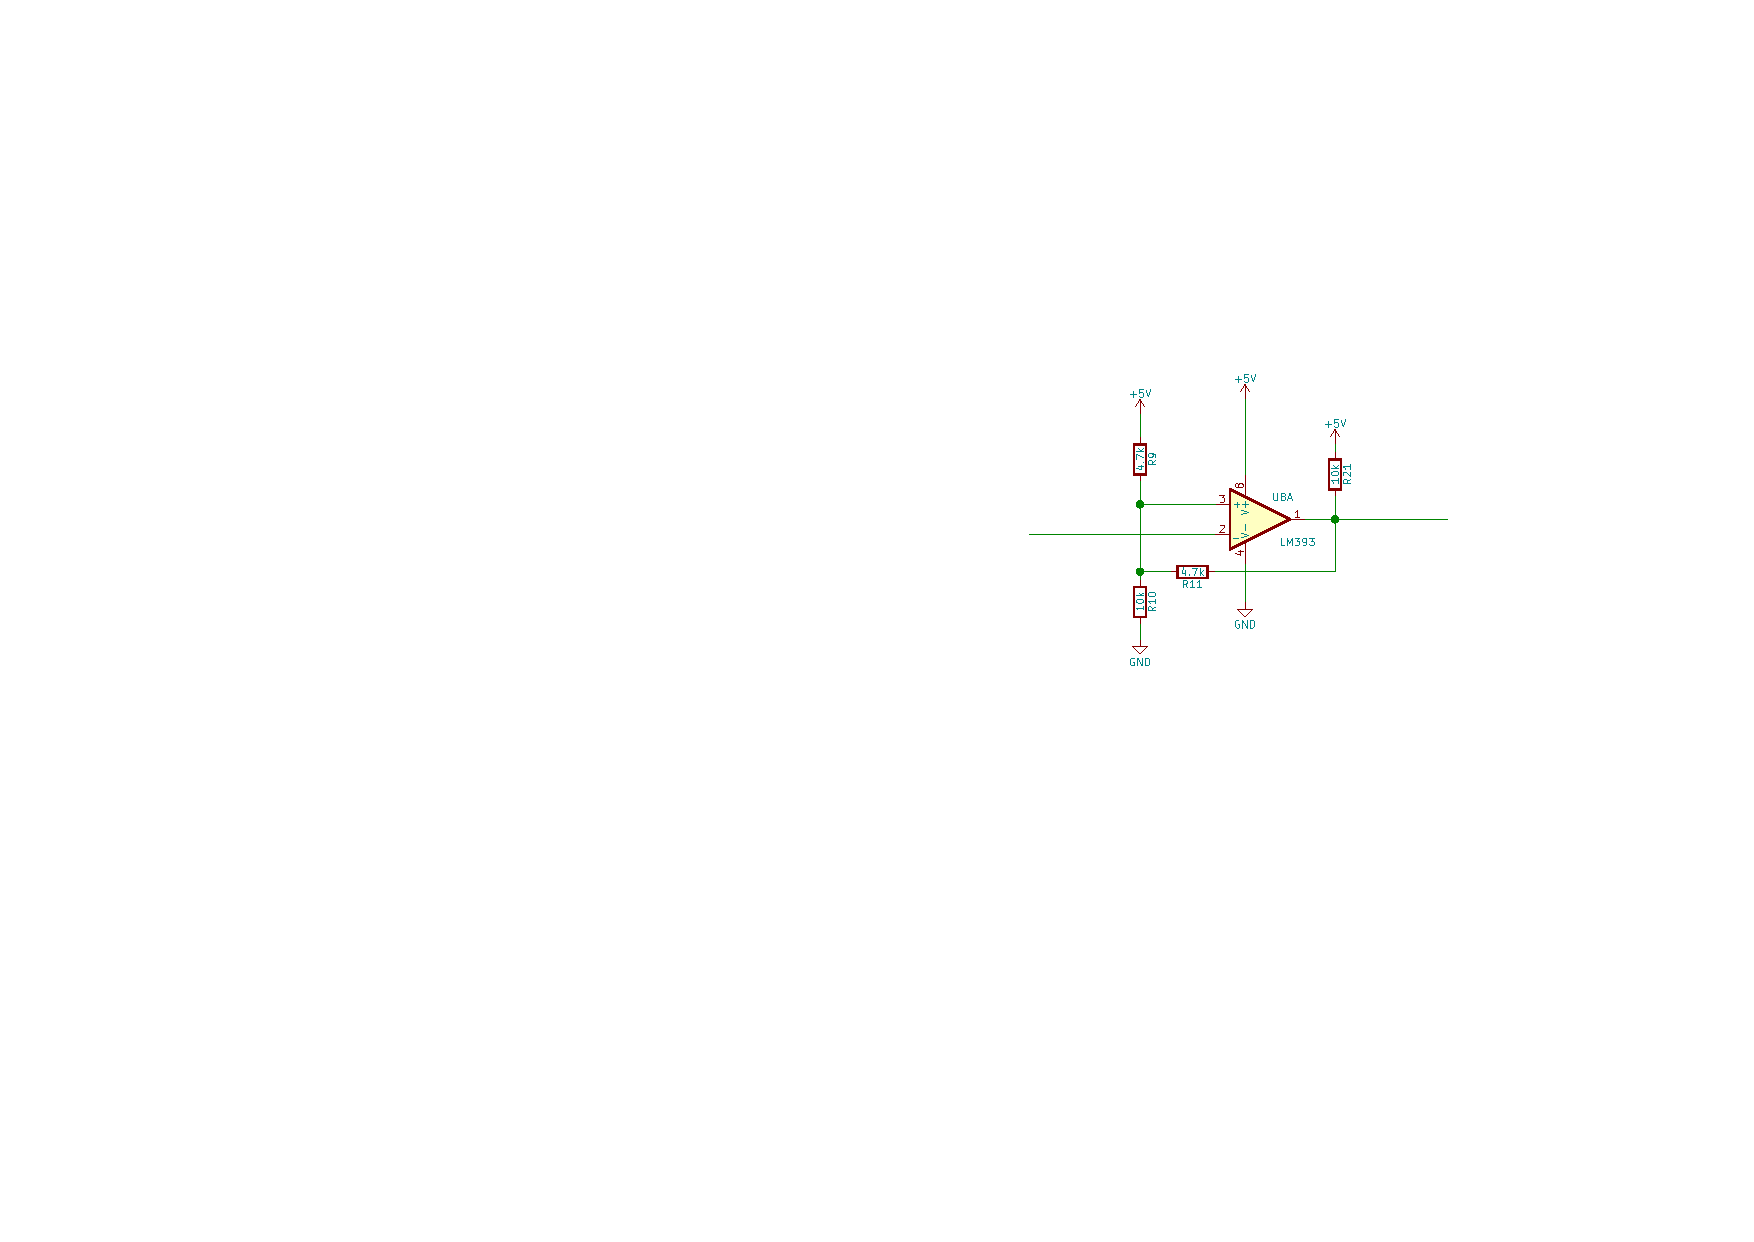
\includegraphics[width=0.4\textwidth]{fig/schmitt_trigger.pdf}
		\end{figure}
\end{description}

\subsection{Décodeur}
Le décodeur à 3 fonctions:

\begin{description}[leftmargin=!,labelwidth=4cm, labelindent=\parindent]
	\item[Down counter] Signal si $n_{pulse}$ impulsions ont été reçues par la tension d'entrée depuis son dernier RESET.
	\item[Missing pulse detector] Signal et reset le down counter après un certain $t_{true} = \SI{5}{\milli\second}$ délais si la tension d'entrée est maintenue \emph{high} pendant au moins $t_{miss} = \SI{1.8}{\milli\second}$ après la fin d'une impulsion. La durée $t_{miss}$ a été arbitrairement choisie pour être supérieur à $t_0 = \SI{1}{\milli\second}$ mais inférieur à $2t_0$. Les dimensionnements sont fait selon le datasheet \cite{TLC555} avec une capacité $\mathit{C3} = \SI{100}{\nano F}$ choisie petite pour la simplicité et la limitation de la consommation.

		\begin{equation*}
			t_{miss} = \mathit{R7}*\mathit{C3} \quad\Rightarrow\quad \mathit{R7} = \SI{18}{\kilo\ohm}
		\end{equation*}

		\begin{figure}[H]
			\centering
			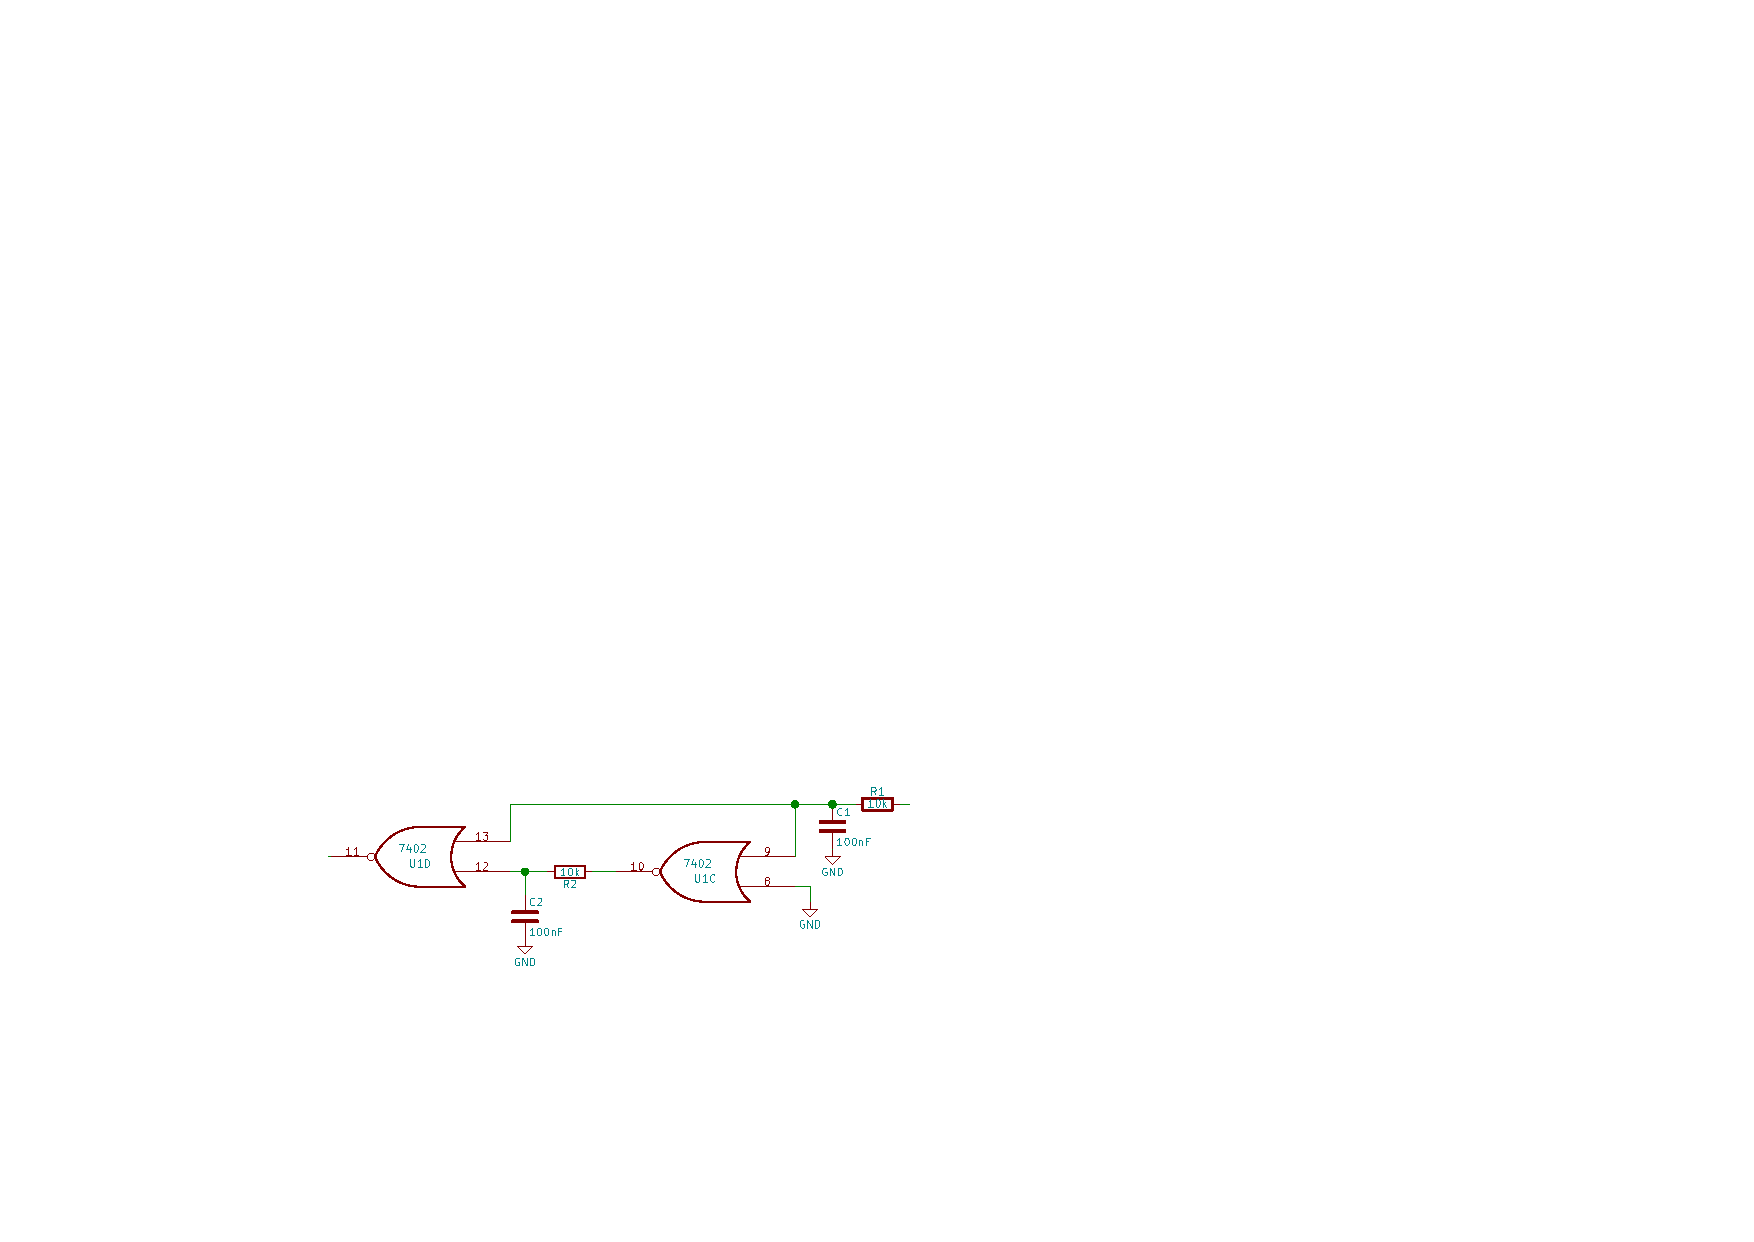
\includegraphics[width=0.4\textwidth]{fig/decoder_reset_delay.pdf}
		\end{figure}

		\todo[inline]{fig decoder\_reset\_delay goto Logic and put fig missing pulse detector instead}

	\item[Logic] Met OUTPUT à high si les conditions d'une salve correcte sont remplie. Si $n_{pulse}$ impulsions ont été reçues et que une impulsion manquante est signalée, alors OUTPUT est mis à high. 

        La logique de sortie est réalisée en NOR gate comme suivant:
        \begin{align*}
        \text{Sortie} & = \text{"bon nombre d'impulsions"} \land \text{"fin de salve"} \\
        & = \overline{\overline{\text{"bon nombre d'impulsions"}} \lor \overline{\text{"fin de salve"}}}
        \end{align*}

\end{description}

\subsection{Sortie}

\begin{description}[leftmargin=!,labelwidth=4cm, labelindent=\parindent]
	\item[Détecteur d'interruption] TODO: valeurs de R et C

    \begin{figure}[H]
    \centering
    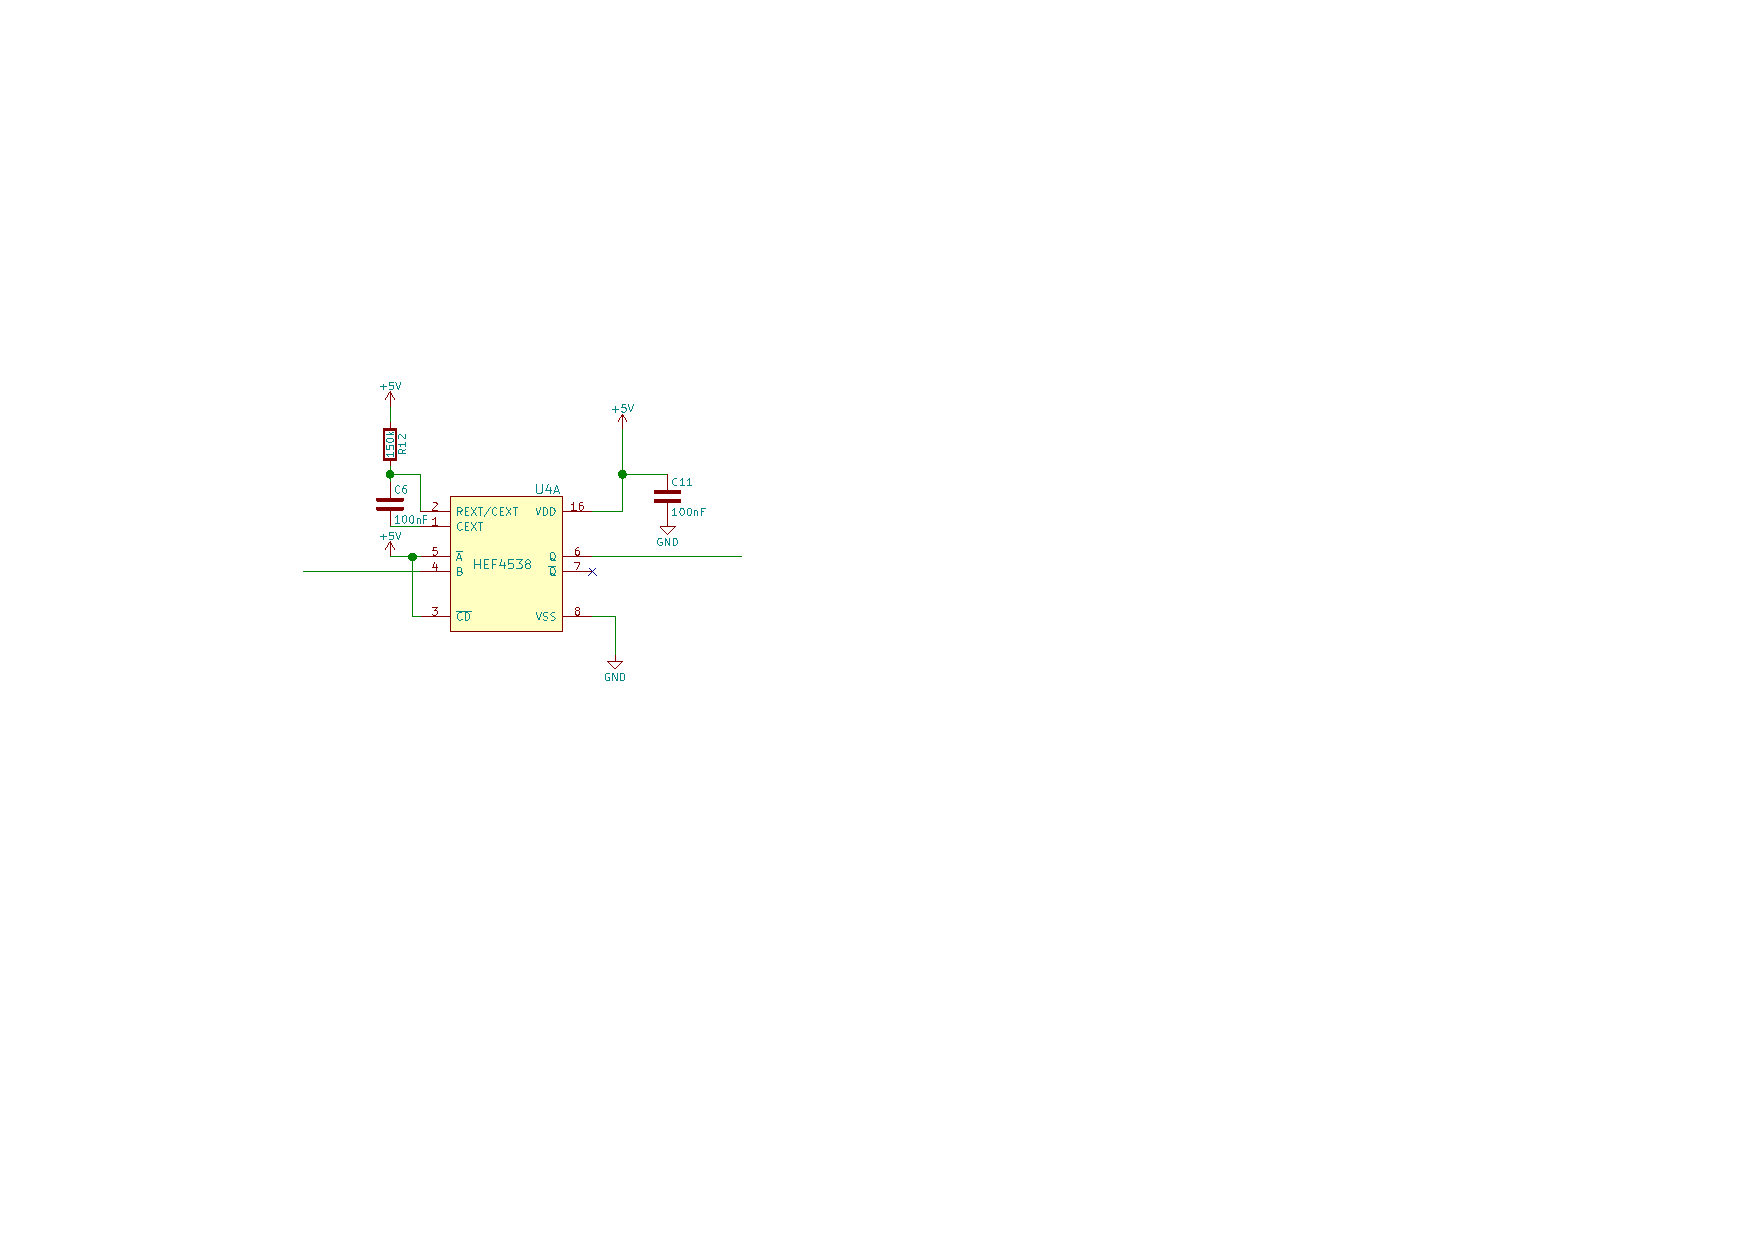
\includegraphics[width=0.4\textwidth]{fig/interrupt_detect.pdf}
    \end{figure}

    \item[Commutateur] TODO: Ce D-flip-flop qui toggle la LED chaque flanc montant...
    % \begin{figure}[H]
    % \centering
    % 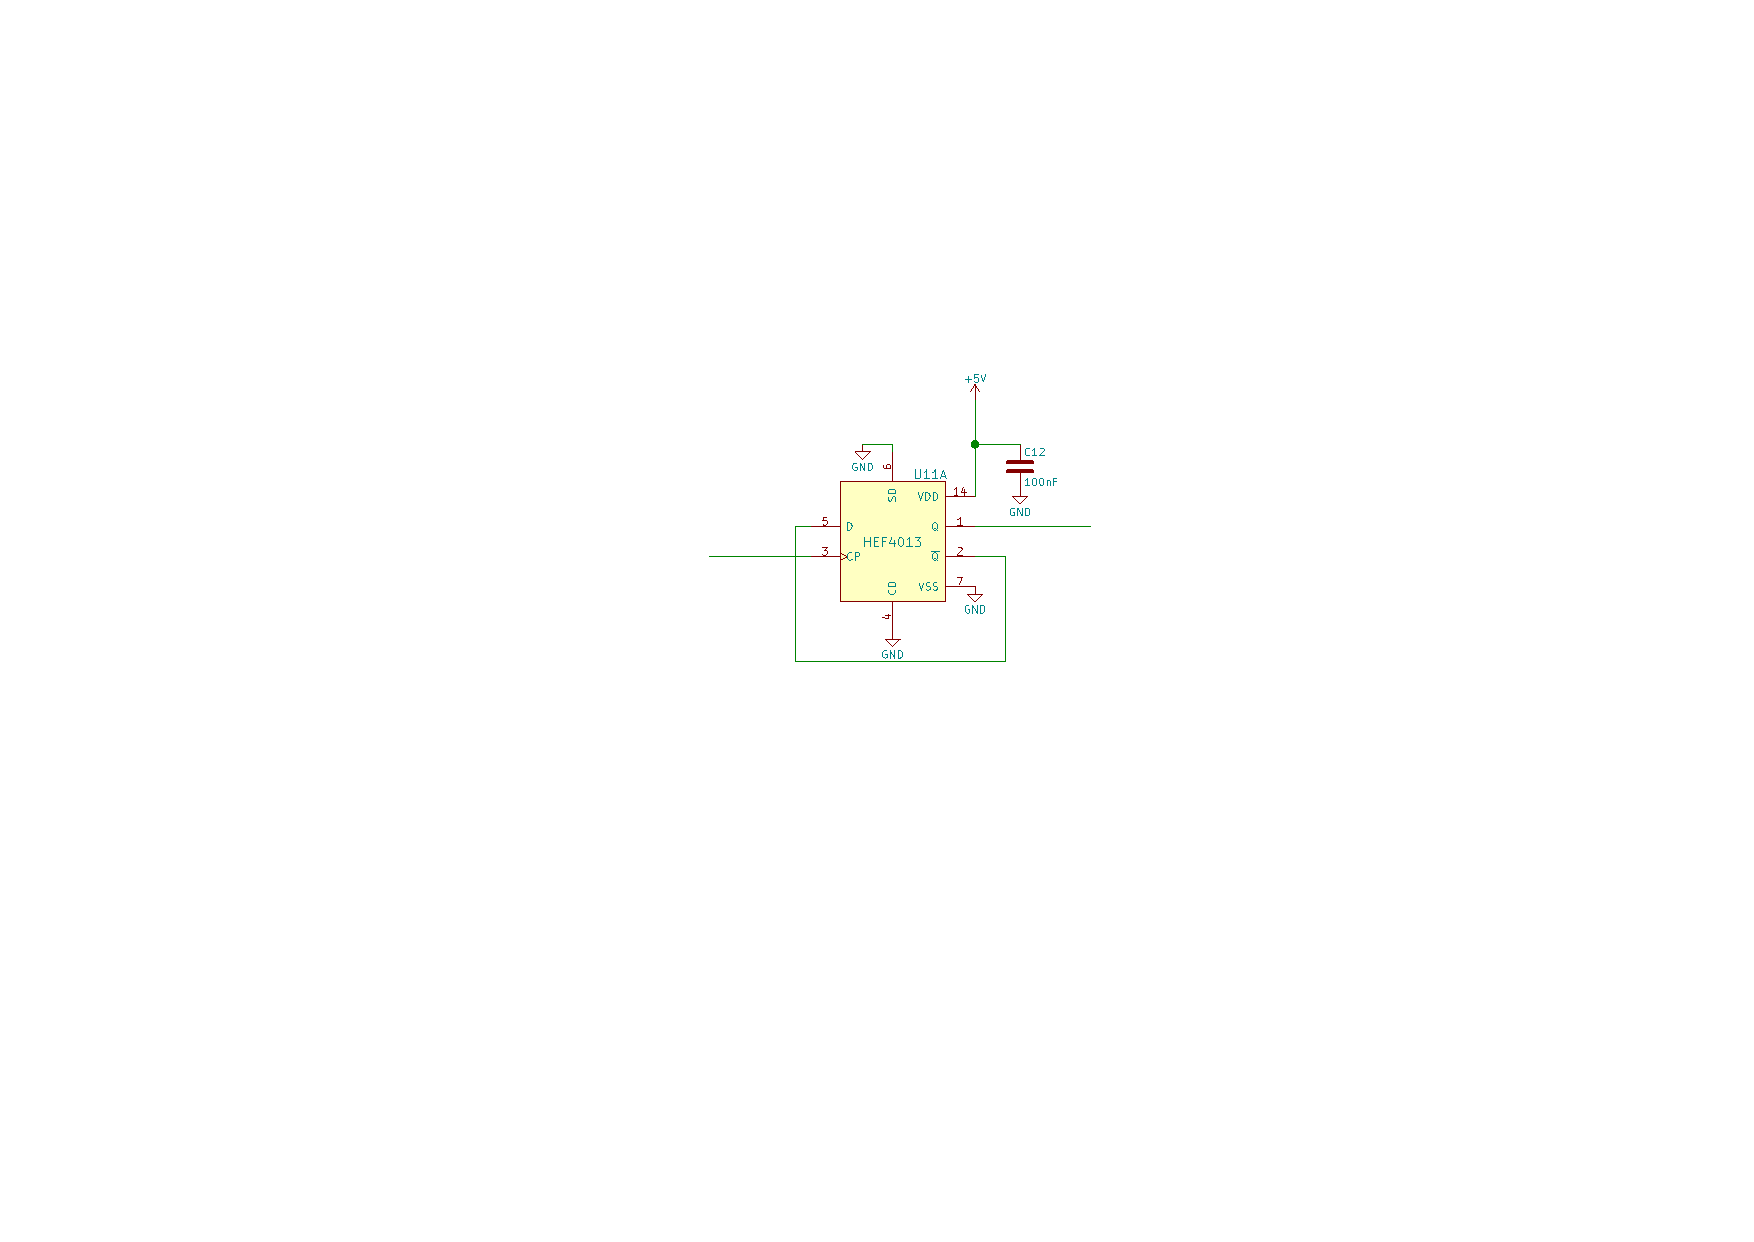
\includegraphics[width=0.4\textwidth]{fig/commutator.pdf}
    % \end{figure}


	\item[Relais] Le relais optique est simulé par une LED rouge standard avec un courant de \SI{20}{\milli\ampere} et une tension directe d'environ \SI{1.8}{\volt}. Pour alimenter la LED on a choisi le transistor bipolaire NPN BC107 avec une résistance en série pour limiter le courant.
		Le BC107 a une tension \(V_{CEsat}\) de \SI{0.25}{\volt} pour un courant de \SI{10}{\milli\ampere}.
		En estimant une \(V_{CEsat}\) de \SI{0.30}{\volt} pour un courant de \SI{20}{\milli\ampere}:

    \begin{equation*}
    R_{LED} = (5V - V_{CEsat} - V_{forward})/\SI{20}{\milli\ampere} = \SI{145}{\ohm} \Rightarrow \SI{150}{\ohm}
    \end{equation*}

    % \begin{figure}[H]
    % \centering
    % 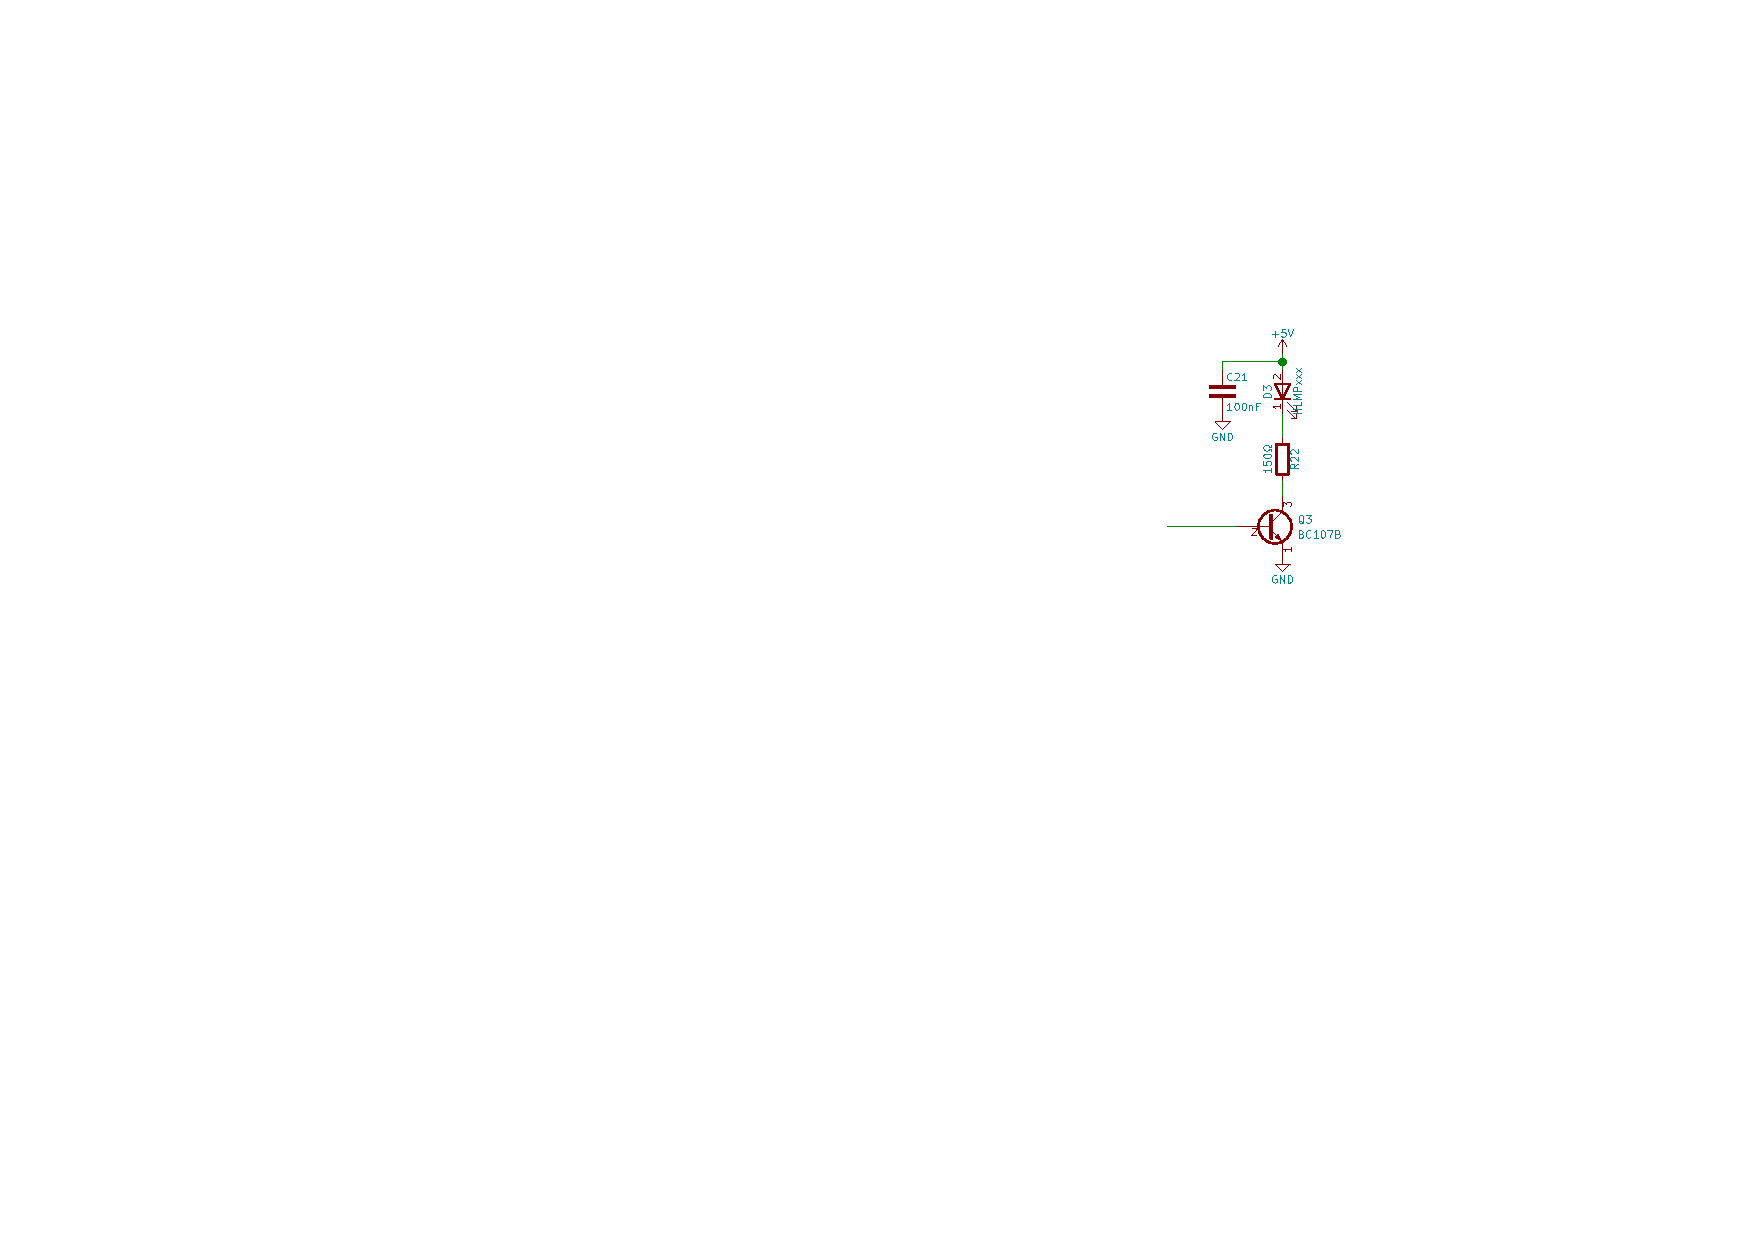
\includegraphics[width=0.2\textwidth]{fig/output_led.pdf}
    % \end{figure}

\end{description}
\subsection{Mesures}

Dans figure \ref{fig:decoder_signal} on voit le fonctionnement du détecteur avec différent nombres d'impulsions.
Dans la mesure au milieu le décodeur détecté correctement les 13 impulsions et la combinaison logique
du signal du détecteur d'impulsion manquant et du compteur d'impulsion donne un signal de sortie (en vert).
Dans le cas où le mauvais nombre  d'impulsions (12 impulsions dans la mesure à gauche et 14 impulsions à droite)
arrive à l'entrée il n'y a pas de signal à la sortie.

\begin{figure}[H]
\centering
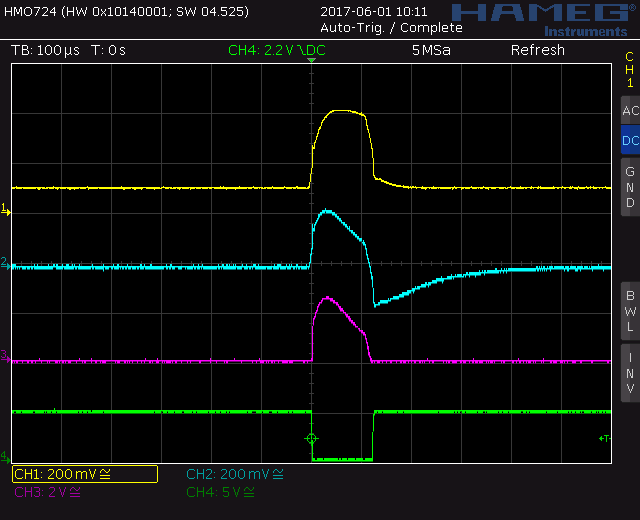
\includegraphics[width=0.3\textwidth]{../measurements/SCR03}
\caption{
\textcolor{yellow}{$\blacksquare$} Conversion courant-tension,
\textcolor{blue}{$\blacksquare$} Filtre passe-haut,
\textcolor{magenta}{$\blacksquare$} Signal 10x amplifié,
\textcolor{green}{$\blacksquare$} Schmitt trigger output
}
\label{fig:filter_signal}
\end{figure}

\begin{figure}[H]
\centering
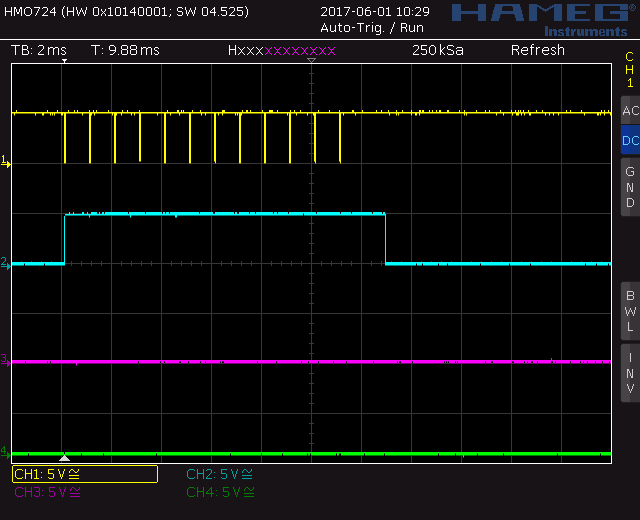
\includegraphics[width=0.3\textwidth]{../measurements/SCR06}
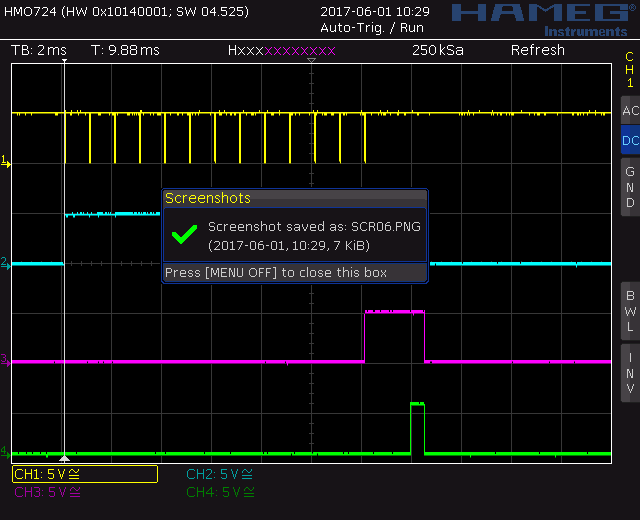
\includegraphics[width=0.3\textwidth]{../measurements/SCR07}
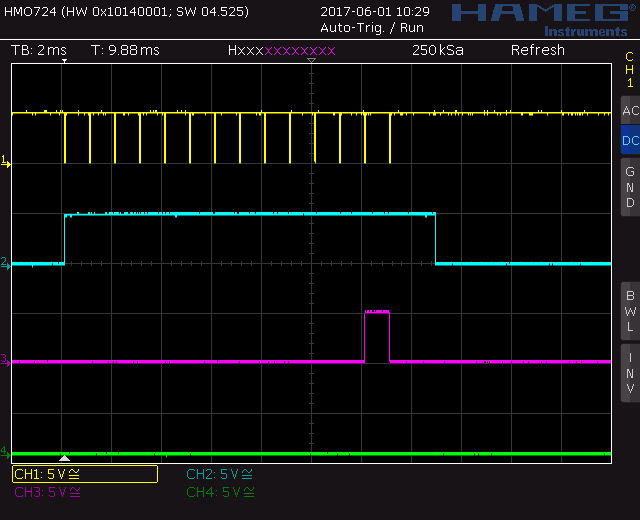
\includegraphics[width=0.3\textwidth]{../measurements/SCR08}
\caption{
\textcolor{yellow}{$\blacksquare$} Signal d'entrée,
\textcolor{blue}{$\blacksquare$} Détecteur d'impulsion manquant,
\textcolor{magenta}{$\blacksquare$} Compteur d'impulsions,
\textcolor{green}{$\blacksquare$} Sortie
}
\label{fig:decoder_signal}
\end{figure}

\begin{figure}[H]
\centering
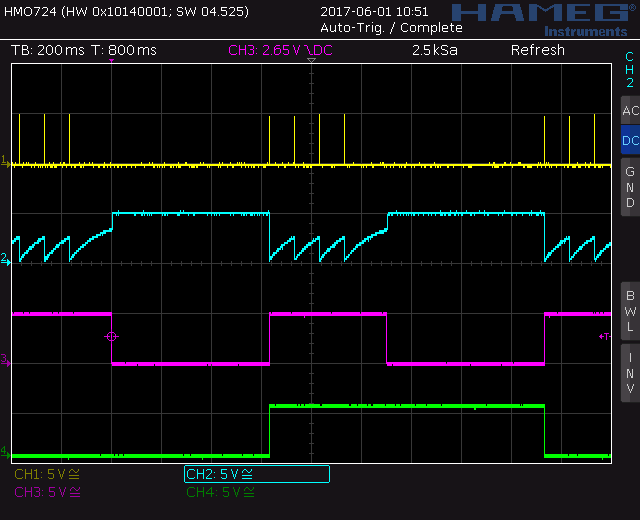
\includegraphics[width=0.3\textwidth]{../measurements/SCR12}
\caption{
\textcolor{yellow}{$\blacksquare$} Signal d'entrée,
\textcolor{blue}{$\blacksquare$} Capacité sur bascule monostable,
\textcolor{magenta}{$\blacksquare$} Sortie du détecteur de pause,
\textcolor{green}{$\blacksquare$} Sortie
}
\label{fig:output_signal}
\end{figure}

\begin{thebibliography}{9}

	\bibitem{LD271(H)}
	OSRAM,
	\textit{LD271 - HGaAs Infrared Emitter},
	Version 1.0,
	4 Avril 2007,
	\url{http://www.osram-os.com/Graphics/XPic5/00082753_0.pdf/LD%20271,%20Lead%20(Pb)%20Free%20Product%20-%20RoHS%20Compliant.pdf}

		\bibitem{BP104}
		VISHAY,
		\textit{BP104 - Silicon PIN Photodiode},
		Revision: 08-Feb-17,\\
		\url{http://www.vishay.com/docs/81500/81500.pdf}

		\bibitem{TLC555}
		TEXAS INSTRUMENTS,
		\textit{TLC555 LinCMOS\texttrademark Timer},
		REVISED AUGUST 2016,
		SEPTEMBER 1983,\\
		\url{http://www.ti.com/lit/ds/symlink/tlc555.pdf}

		\bibitem{HEF4526B}
		NXP,
		\textit{HEF4526B - Programmable 4-bit binary down counter - Product data sheet},
		Rev. 5,
		22 November 2011,\\
		\url{http://www.nxp.com/documents/data_sheet/HEF4526B.pdf}.

		\bibitem{HEF4001B}
        NXP,
        \textit{HEF4001B - Quad 2-input NOR gate - Product data sheet},
        Rev. 10,
        10 December 2015,\\
        \url{https://assets.nexperia.com/documents/data-sheet/HEF4001B.pdf}

        \bibitem{IRLU8259}
        International Rectifier,
        \textit{IRLU8259PbF - HEXFET\textregistered Power MOSFET},
        PD - 97360,
        16 December 2008,\\
        \url{http://www.infineon.com/dgdl/irlr8259pbf.pdf?fileId=5546d462533600a40153566e1ebe26e9}

        \bibitem{LMC6482}
		Texas Instruments,
		\textit{LMC6482 CMOS Dual Rail-to-Rail Input and Output Operational Amplifier},
		SNOS674E,
		April 2015,\\
		\url{http://www.ti.com/lit/ds/symlink/lmc6482.pdf}

\end{thebibliography}

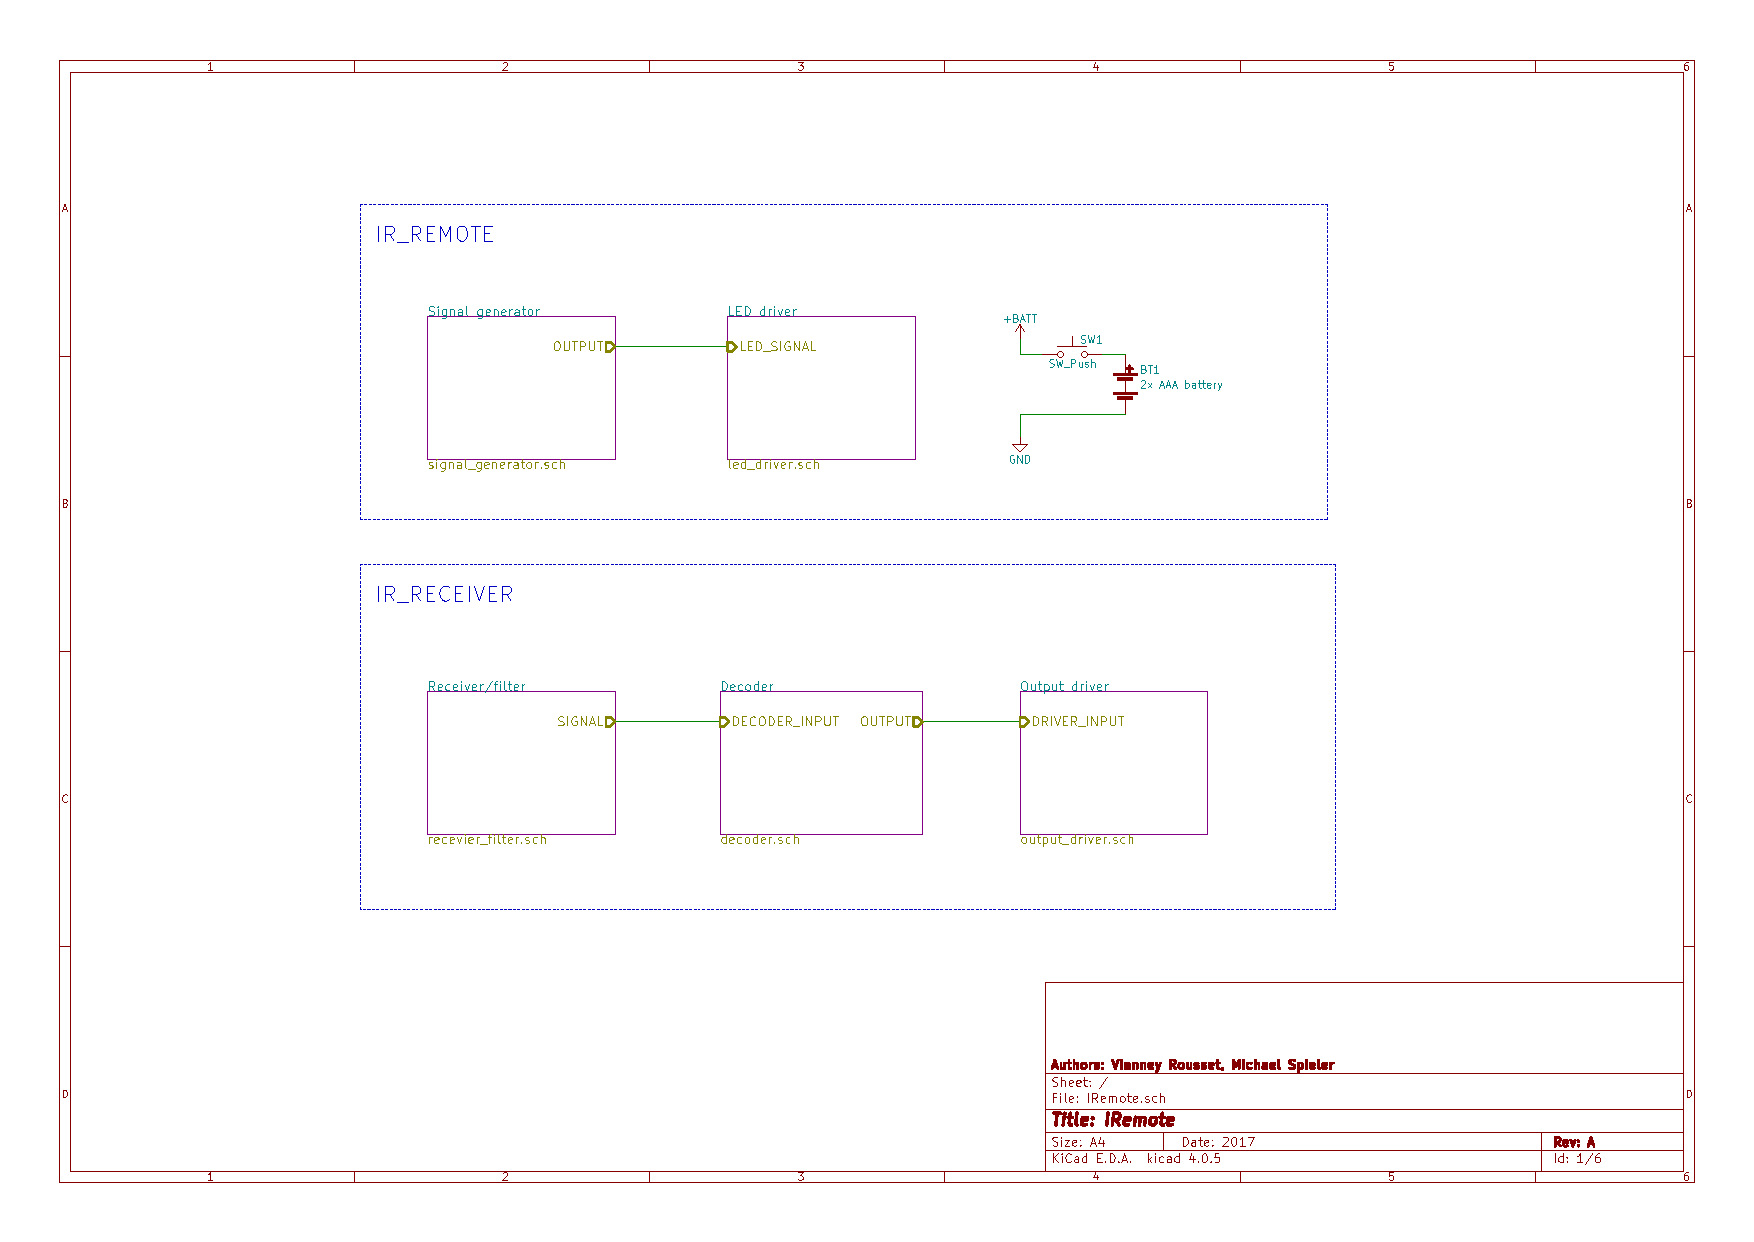
\includepdf[pages={-},angle=90,scale=0.95,pagecommand={}]{../schema/IRemote.pdf}

\end{document}
